\section{tasks::adjustwave Class Reference}
\label{classtasks_1_1adjustwave}\index{tasks::adjustwave@{tasks::adjustwave}}
Inheritance diagram for tasks::adjustwave::\begin{figure}[H]
\begin{center}
\leavevmode
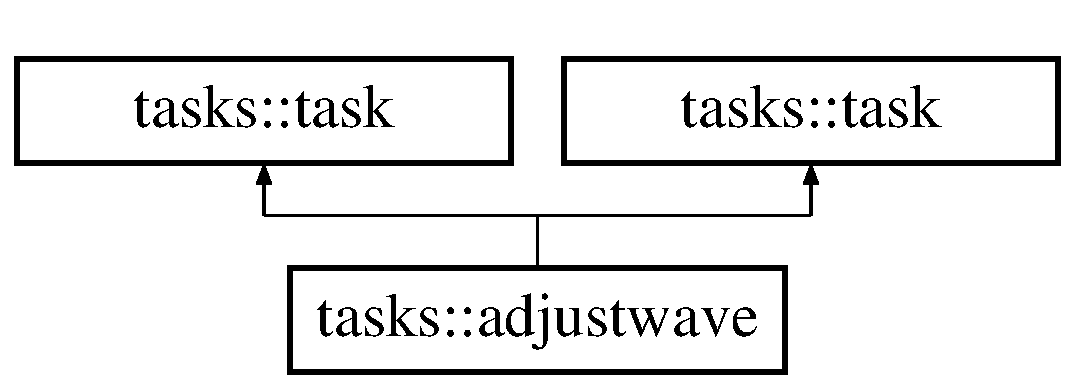
\includegraphics[height=2cm]{classtasks_1_1adjustwave}
\end{center}
\end{figure}
\subsection*{Public Member Functions}
\begin{CompactItemize}
\item 
def \textbf{run}\label{classtasks_1_1adjustwave_9621b453303f59a928546f58694201e2}

\item 
def \textbf{run}\label{classtasks_1_1adjustwave_9621b453303f59a928546f58694201e2}

\end{CompactItemize}
\subsection*{Static Public Attributes}
\begin{CompactItemize}
\item 
string \textbf{name} = '{\bfadjustwave}'\label{classtasks_1_1adjustwave_d2328aa56edd2173869ce6a65e506f4e}

\item 
string \textbf{button\-Text} = 'Adjust wavelengths'\label{classtasks_1_1adjustwave_05f4e1d2dc42a15e1973c552b20c3fda}

\item 
string \textbf{suffix} = 'adjwave'\label{classtasks_1_1adjustwave_6e46604461307022021de2eb12048deb}

\item 
list \textbf{prereq} = ['{\bfgetspecshift}', '{\bfaddwave}']\label{classtasks_1_1adjustwave_11e5a718bb52e59001ffdcb9d4d294a1}

\end{CompactItemize}


\subsection{Detailed Description}


\footnotesize\begin{verbatim}Adjust the wavelength definition by correcting for possible shifts in the
   simultaneously observed interlaced calibration lamp spectrum.
\end{verbatim}
\normalsize
 



The documentation for this class was generated from the following files:\begin{CompactItemize}
\item 
old/PANICtool-1.0/tasks.py\item 
old/tasks.py\end{CompactItemize}
